\section{Evaluation}
In order to determine success, applicability, and weak-points of the CubanSea design, a user study has been undertaken consisting of an assessment and an online survey, trying to compare CubanSea to traditional search engines. A total of ten users contributed to this study. Six users participated in the verbal assessment, seven in the survey. Two users provided incorrect or incomplete filled-out survey sheets, while five users completed the online survey successfully. Four small tasks of gathering urls of web sites relevant to a specified search query and of extracting information hidden within the documents of the result space were defined. Two groups were created, each performing two tasks with their acquired search engine and two using CubanSea. The time and correctness was measures. Furthermore, users were asked to answer subjective questions on what they thought about the systems, to assess their quality, and to compare them with one another. Maybe unsurprisingly, all users identified Google as their commonly used search engine.

The primary criteria for CubanSea is the aided recognition of relevant search results. For this, time and correctness of the undertaken tasks are critical. The results gathered by measuring the time revealed a surprising success. Task completion was much faster than when using Google. Figure \ref{fig:eval:time} displays the results. Using CubanSea, users required in average only 43.1\% of the time they needed using Google for completing the exact same task. This result is specifically interesting since CubanSea is only a prototype running on a low performance machine, thus making CubanSea considerably slower than the speed optimized Google Search.
\begin{figure}[!t]
	\centering
	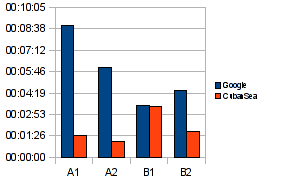
\includegraphics[width=3in]{evaluation-time}
	\caption{Average required time to complete task}
	\label{fig:eval:time}
\end{figure}
No difference could be recorded in result quality. Only two results were erroneous, both coming from task B1: one was created using Google, one using CubanSea. Further studies would be helpful determining the individual impact on these results for the different technologies used in the CubanSea visualization.

Besides collecting empiric data, the users also had to answer questions on their subjective satisfaction with both Google and CubanSea, as well as compare the two engines with one another. This subjective happyness is crucial for the success of a search engine. No visualization can ever hope of being successfully accepted if users are not comfortable using it. The results were inconclusive. Even though CubanSea recieved in average better ratings, most of the answer space overlapped. Users exist both liking and disliking either one of the interfaces. No connection could be discovered between user preference and personal user data such as age, gender, cultural background, occupation, or experience with computers. Figure \ref{fig:eval:happyness} displays the result distribution for the question ``how happy are you with Google / CubanSea''.
\begin{figure}[!t]
	\centering
	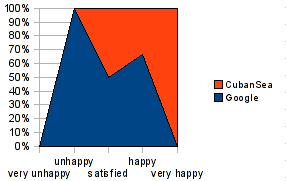
\includegraphics[width=3in]{evaluation-happyness}
	\caption{User happiness distribution}
	\label{fig:eval:happyness}
\end{figure}

During the assessments, users were guided through the process of using the interface application. Those users participating in both the assessments and the survey took the survey first. Users were asked to perform two tasks of their choice from the survey by using CubanSea. While doing so, their actions were observed and feedback was gathered. Three of six users initially wanted to reformulate their query. One user had trouble understanding the meaning of the different topics presented in the overview. Most users (67\%) criticized the performance of the system which was to be expected due to the nature of the experimental deployment. Otherwise, all users subjectively liked the system. Specifically the filter functionality was highly praised.

Two users criticized the fact that only the first five result snippets were initially visible. They suggested the initial display of all snippets. Interestingly, both users had previously replied to the question on where they would usually find their search results with ``within the first few results returned by a search engine''. It would have been expectable that those users wouldn't need the other results and thus not their snippets. Further studies should be undertaken to evaluate the potential benefit of hiding the snippets from all results but the first five.

Users also criticized that the clustering algorithm did not prevent result items from being assigned to the wrong topic. In order to correct this, additional research is required optimizing the clustering algorithm. The general visualization of the different topics, however, was accepted. Errors were encounterd in the automated collapse of clusters. Regularily, clusters that obviously deal with identical topics are not discovered to be the same, but are maintained as two separate topics. Also, the topic header generation sometimes yields ambigouos topic names.

The overall result of the use case study was very positive and encouraging. The visualization successfully aids in the process of performing search tasks, reducing the required time without compromising the result quality. The interface recieved in average higher ratings regarding the user satisfaction than traditional search engines and no critical weak-point was discovered.